%----------------------------------------------------------
\def\notedate{2022.10.15}
\def\currentauthor{Василян А.Р. (РК6-73Б)}
%----------------------------------------------------------
\notestatement{rndhpcgui}{Методический подход к созданию универсального пользовательского интерфейса}

%---------------------------------------------------------
	На рисунке ~\ref{scheme1} представлены составные элементы подхода к созданию универсального средства построения пользовательского интерфейса программных средств.

\begin{figure}[!ht]
  \centering
  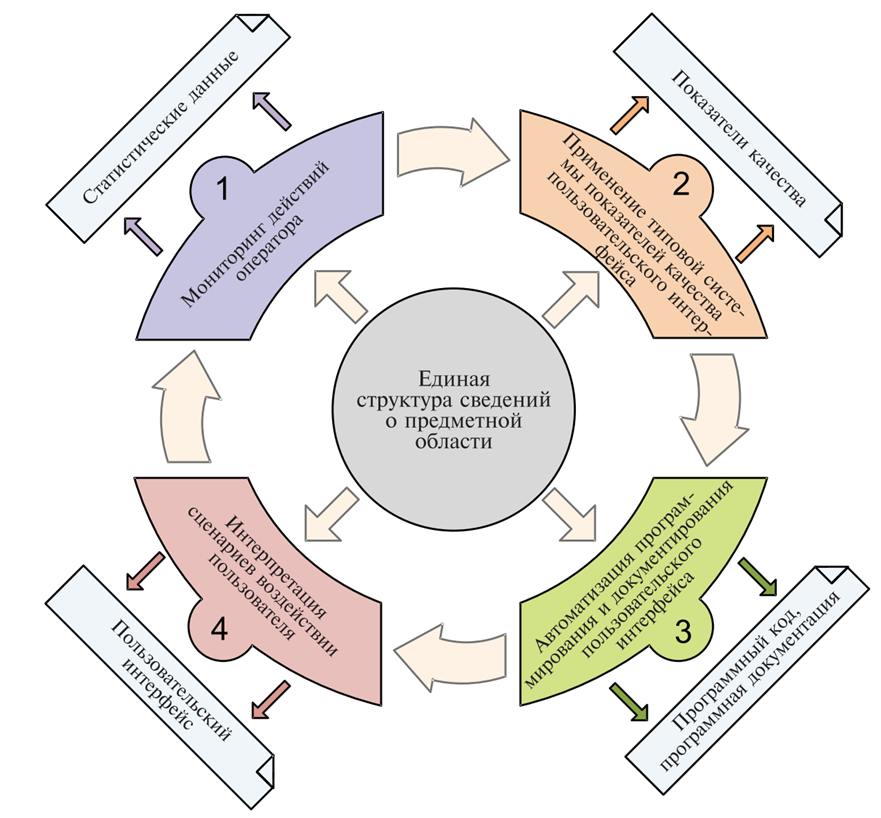
\includegraphics[scale=0.8]{ResearchNotes/rndhpc_not_gui_2022_10_15/scheme1.png}
  \caption{Составные элементы подхода к созданию универсального средства построения пользовательского интерфейса программных средств}
  \label{scheme1}
\end{figure}

	Мониторинг действий оператора (блок 1 на рис. ~\ref{scheme1}) позволяет осуществлять сбор и накопление статистики деятельности оператора во время эксплуатации программных средств. Оператор вводит входные параметры с помощью технических средств ввода данных: клавиатуры, манипулятора «мышь», фотокамеры, микрофона, сканера, специализированных панелей кнопок и переключателей, внешних носителей информации и т. п. Каждая атомарная операция основывается на низкоуровневых сигналах от средства ввода, преобразуемых программной средой в воздействия ввода оператора за счет событийной обработки.
Оценка качества пользовательского интерфейса обеспечивается за счет:
\begin{itemize}
	\item применения типовой системы показателей качества (блок 2 на рис. ~\ref{scheme1});
	\item разработки методики оценки качества;
	\item выполнения мероприятий по оценке показателей качества.
\end{itemize}

	Система показателей качества пользовательского интерфейса основывается на сведениях представленных типов:
\begin{itemize}
	\item аппаратные события – события, которые возникают от действия всех технических средств при работе с периферийным оборудованием, а также вследствие использования каналов связи и удаленных подключений;
	\item события приложения – события, связанные с операциями получения, обработки и преобразования данных, обеспечения политики безопасности и уровней доступа, т. е. все эти события появляются в процессе функционирования программы в программной среде;
	\item пользовательские события – события, предусмотренные программой, происходят в результате воздействий пользователя на элементы управления интерфейса.
\end{itemize}

	Величины, с помощью которых можно определить качество выполнения операции:
\begin{itemize}
	\item среднее время выполнения операции; 
	\item число ошибок (количество итераций), возникающих за период работы;
	\item среднее время возникновения ошибки.
\end{itemize}

	Показатели качества пользовательского интерфейса выражаются в формате: 
\begin{itemize}
	\item время выполнения операций (действий); 
	\item число действий, необходимых для выполнения операции; 
	\item число атомарных операций, необходимых для выполнения действия; 
	\item число пустых воздействий, выполненных оператором; 
	\item число ошибочных атомарных операций.
\end{itemize}

	"Автоматизация программирования и документирования пользовательского интерфейса" (блок 3 на рис. ~\ref{scheme1}) подразумевает возможность автоматизированного документирования интерфейса программы.
	Основные мероприятия жизненного цикла пользовательского интерфейса: 
\begin{itemize}
	\item задание требований; 
	\item проектирование; 
	\item разработка, программирование
	\item оценка качества и испытания; 
	\item документирование (описание).
\end{itemize}

	Каждое мероприятие жизненного цикла интерфейса взаимосвязано с UML моделями, описывающими интерфейс, которые в ходе итерационного процесса разработки корректируются и используются для получения документов.
	В соответствии с подходом предусматривается автоматизация программирования макетов пользовательского интерфейса, основанная на таком выборе паттерна проектирования программного кода, который позволит инкапсулировать механизмы обработки данных и управления от элементов управления интерфейса, но при этом обеспечит связь с моделью данных и мониторинг действий оператора.
	Можно использовать UML модель сценариев применения пользовательского интерфейса (модель сценариев воздействий пользователя (СВП)), описывающая различные стороны функционирования программы, которая выражает на определенном уровне абстракции порядок взаимодействия пользователя с программным средством. Модель используется для декомпозиции и формирования однозначного понимания сведений по совокупности функций и режимов работы разрабатываемого программного средства, а также для обеспечения возможности автоматизированного документирования и построения кода интерфейса программы.

	С помощью UML модели СВП решаются следующие задачи: 
\begin{itemize}
	\item прототипирование и/или макетирование пользовательского интерфейса при разработке программного средства;
	\item формализация существующего пользовательского интерфейса;
	\item описание деятельности пользователя при эксплуатации программных средств, выраженное в виде набора осуществленных сценариев воздействий на элементы управления программы.
\end{itemize}

	Отображение некоторого абстрактного сценария осуществляет механизм его интерпретации (блок 4 на рис. ~\ref{scheme1}) в стандартные программные процедуры, характерные для выбранной программноаппаратной платформы. Наличие интерпретатора предписывает применение некоторой формальной логики (языка), с помощью лексем которой выражаются любые сценарии. Одна лексема описывает типовую атомарную операцию над элементом управления пользовательского интерфейса, идентифицирующие сведения о которой содержатся в параметрах лексемы.
	Каждая атомарная операция, которая вызвана воздействиями пользователя, на диаграмме СВП представляет собой дугу графа, вершины графа — элементы управления пользовательского интерфейса, веса графа — комплексные показатели, характеризующие:
\begin{itemize}
	\item количество выполнений атомарной операции; 
	\item время выполнения атомарной операции;
	\item количество ошибок, связанных с выполнением атомарной операции.
\end{itemize}
%----------------------------------------------------------
% Атрибуты задачи
\noteattributes{}
%----------------------------------------------------------

